Zum Vergleich der im  Kapitel \emph{Fehlerrechnung} bestimmten Durchflusswerte
mit   den  eingestellten   Werten   sei  hier   noch   die  Unsicherheit   des
Durchflussmessers ber\"ucksichtigt, welche  gem\"ass Versuchsanleitung \SI{\pm
0.01}{\liter\per\minute} betr\"agt.

Die  Abbildungen   \ref{fig:results:laminar}  und  \ref{fig:results:turbulent}
zeigen   graphische  Vergleiche   zwischen  eingestellten   und  experimentell
bestimmten  Werten,   Tabelle  \ref{tab:finalresults}  fasst   die  Ergebnisse
tabellarisch zusammen.

\begin{table}[h!t]
    \centering
    \caption{%
        Durchflussraten. Vergleich  experimentelle Resultate  und Angaben  des
        Durchflusssensors.
    }
    \label{tab:finalresults}
    \begin{tabular}{>{\raggedright}p{30mm}SS}
        \toprule
        Versuch
        & {Experiment(\si{\liter\per\minute})}
        & {Durchflusssensor (\si{\liter\per\minute})}
        \\
        \midrule
        laminares Str\"omungsprofil
        & 0.54 \pm 0.02
        & 0.56 \pm 0.01
        \\
        turbulentes Str\"omungsprofil
        & 6.8 \pm 0.3
        & 7.0 \pm 0.01
        \\
        \bottomrule
    \end{tabular}
\end{table}

\pgfplotsset{try min ticks = 4}
\begin{figure}[ht!]
    \centering
    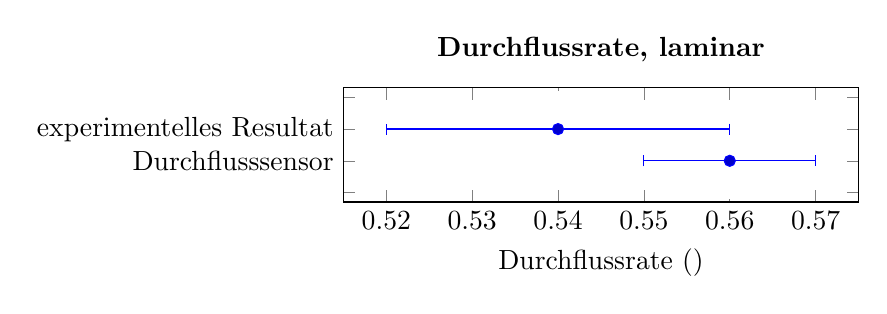
\begin{tikzpicture}
        \begin{axis}[
            %hide y axis,
            width=.67\textwidth,
            height=.25\textwidth,
            title = {\textbf{Durchflussrate, laminar}},
            xlabel = {Durchflussrate ($\si{\liter\per\minute}$)},
            symbolic y coords = {\textcolor{white}{a},Durchflusssensor,experimentelles Resultat,\textcolor{white}{b}},
        ]
        \addplot+[
            only marks,error bars/.cd,
            x dir=both,x explicit,
            error bar style={line width=0.5pt},
            ]
        coordinates {
            (0.54,experimentelles Resultat) +- (0.02,0)
            (0.56,Durchflusssensor) +- (0.01,0)
        };
        \addplot+[
            only marks,
            mark options={color=white},
            color=white,
        ]
        coordinates {
            (0.54,\textcolor{white}{b})
            (0.56,\textcolor{white}{a})
        };
        \end{axis}
    \end{tikzpicture}
    \caption{Vergleich Durchflusssensor und experimentelles Resultat, laminare Str\"omung}
    \label{fig:results:laminar}
\end{figure}

\pgfplotsset{try min ticks = 4}
\begin{figure}[ht!]
    \centering
    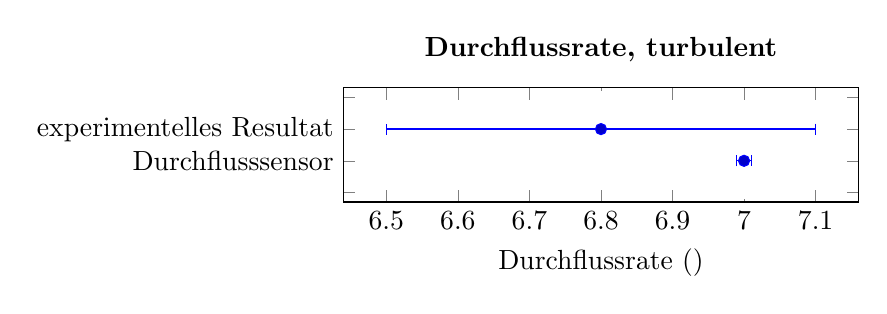
\begin{tikzpicture}
        \begin{axis}[
            %hide y axis,
            width=.67\textwidth,
            height=.25\textwidth,
            title = {\textbf{Durchflussrate, turbulent}},
            xlabel = {Durchflussrate ($\si{\liter\per\minute}$)},
            symbolic y coords = {\textcolor{white}{a},Durchflusssensor,experimentelles Resultat,\textcolor{white}{b}},
        ]
        \addplot+[
            only marks,error bars/.cd,
            x dir=both,x explicit,
            error bar style={line width=0.5pt},
            ]
        coordinates {
            (6.8,experimentelles Resultat) +- (0.3,0)
            (7.0,Durchflusssensor) +- (0.01,0)
        };
        \addplot+[
            only marks,
            mark options={color=white},
            color=white,
        ]
        coordinates {
            (6.8,\textcolor{white}{b}) +- (0.3,0)
            (7.0,\textcolor{white}{a}) +- (0.3,0)
        };
        \end{axis}
    \end{tikzpicture}
    \caption{Vergleich Durchflusssensor und experimentelles Resultat, turbulente Str\"omung}
    \label{fig:results:turbulent}
\end{figure}

In beiden  F\"allen kann eine  ziemlich gute \"Ubereinstimmung  von Experiment
und Referenzwert festgestellt werden. Alles in Allem beurteile ich den Versuch
somit als Erfolg.
